\chapter{Background}
\label{ch:Background} 

%\section{RISC-V}
%
%\textbf{TODO: basic forklaring av RISC-V. Mulig det fra introdksjonen holder?}
%
%In RISC-V, the state of the processor is stored in multiple types of registers. The 32 \textit{general purpose registers (GPR)} are visible to the programmer in the unprivileged mode, are used for normal program execution, and are read and written to by the instructions \cite{waterman_risc-v_2019}. Additionally, the \textit{program counter (PC)} is the register that holds the address of the current instruction \cite{waterman_risc-v_2019}. There is also a set of registers that are typically inaccessible to the programmer in the unprivileged mode. These \textit{Control and Status Registers (CSR)} are used to control and monitor the operation of the processor.
%
%\section{Pipeline \& Interrupts}
%\label{sec:interrupts}

%\section{RISC-V}
%
%\tmp{Holder det som står i introduksjon?}
%
%\tmp{TODO: Registers, CSRs, instruction types}


\section{Pipeline}
\label{sec:bg_pipeline}

Almost all of today's processor cores use pipelining to some extent to increase the throughput and reduce the cycle times of the processor. RISC-V has also been specifically designed for pipelined execution \cite{pattersonComputerOrganizationDesign2021}. 
Typically, an in-order RISC-V pipeline has five steps \cite{pattersonComputerOrganizationDesign2021}:

\begin{itemize}
    \item \textbf{IF} - Fetch instructions from memory
    \item \textbf{ID} - Decode instruction and read registers
    \item \textbf{EX} - Execute the operation and calculate the memory address
    \item \textbf{MEM} - Read/write to the data memory
    \item \textbf{WB} - Write back the result from an operation to a register
\end{itemize}

\subsection{CV32E40S Pipeline}
\label{sec:bg_cv32Pipeline}


\begin{figure}[htb]
    \centering
    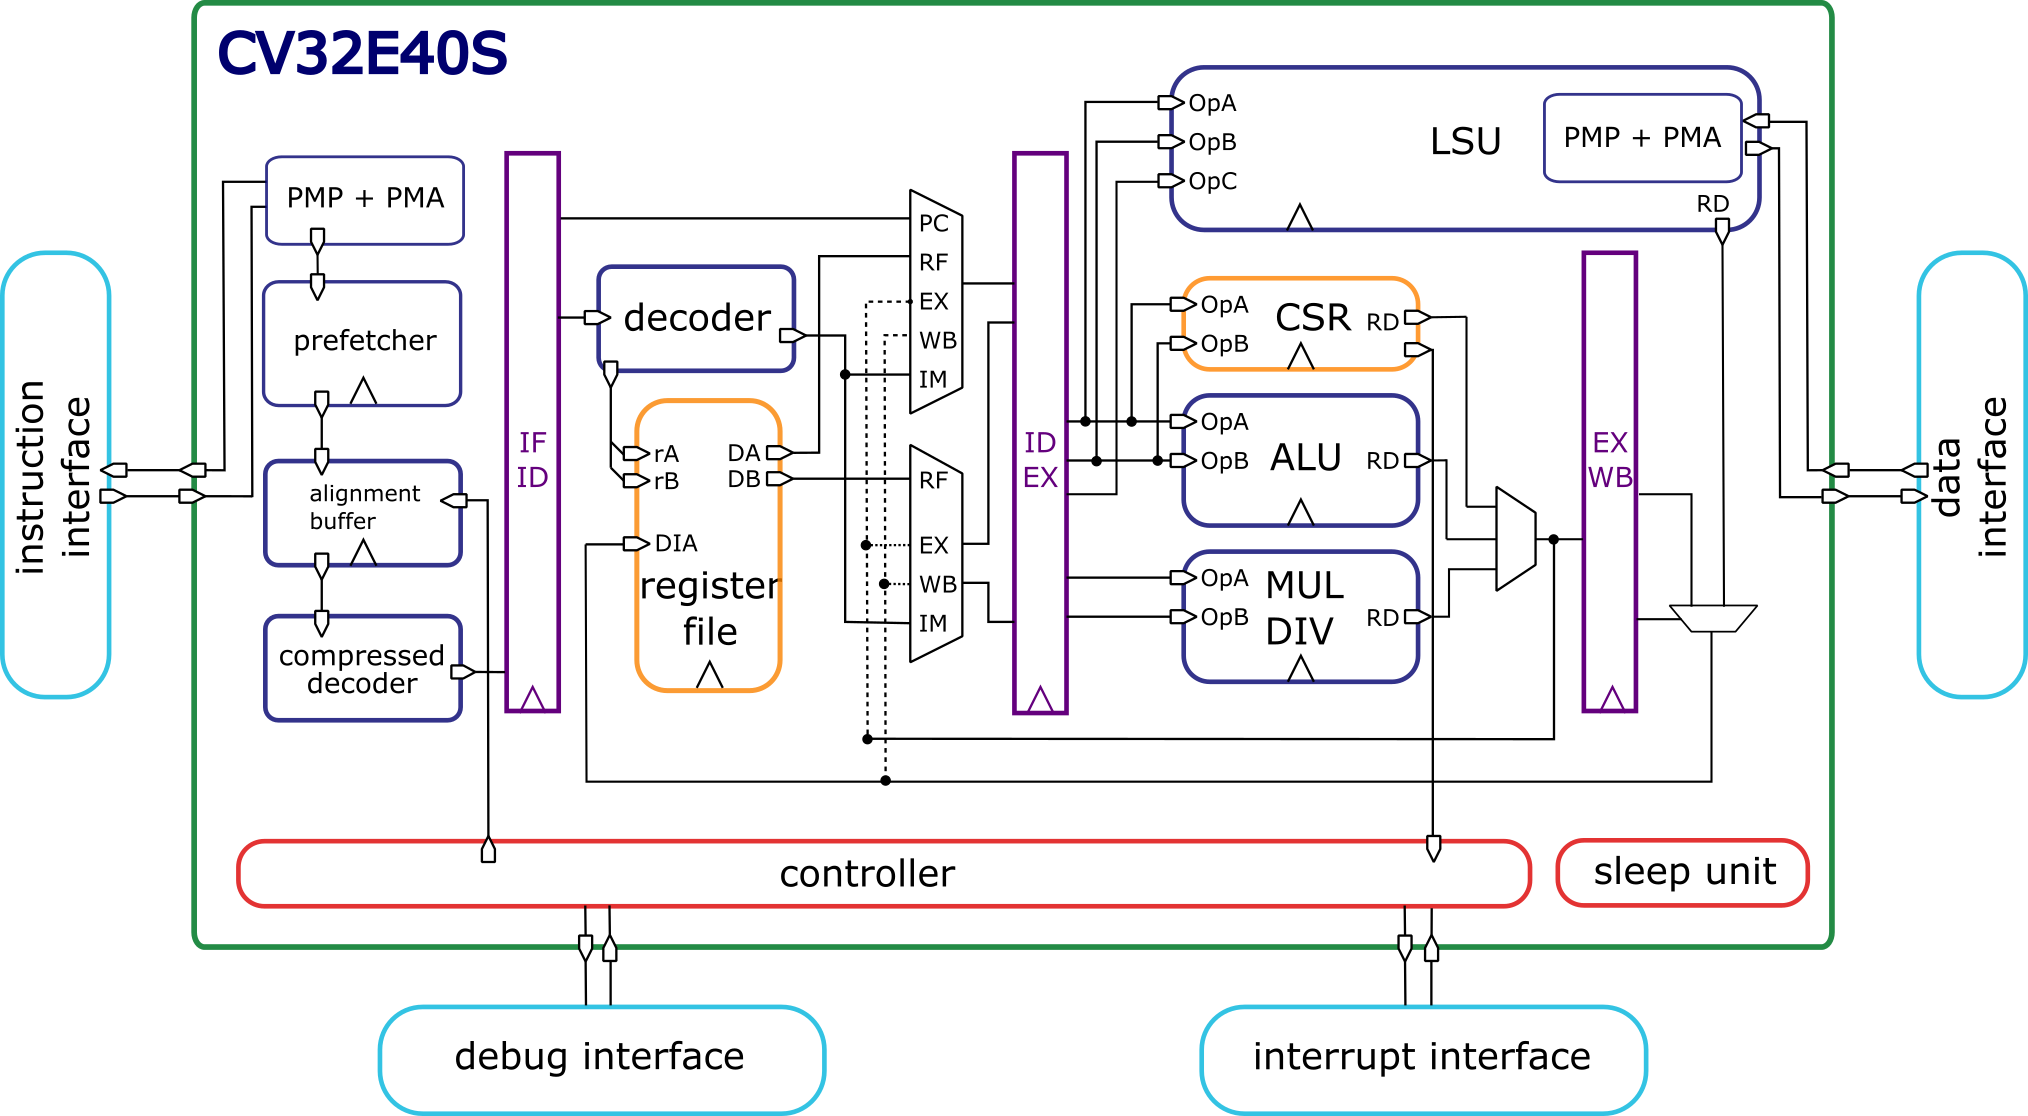
\includegraphics[width=\linewidth]{figures/CV32E40S_Block_Diagram.png}
    \caption{Block diagram of the CV32E40S RISC-V Core from \cite{openhwgroupIntroductionCOREVCV32E40S2023}.}
    \label{fig:cv32e40s-block}
\end{figure}

\Cref{fig:cv32e40s-block} shows a block diagram of the components and pipeline registers of the CV32E40S core from OpehHW Group.
The figure shows that the CV32E40S differs from the standard pipeline because it only has four pipeline stages. To achieve this, the \acrlong{lsu} responsible for loading and storing data from memory is divided so that the address generation is done in the EX stage, and the result is received in the WB stage.
The responsibilities of the four stages are explained below.

\subsubsection{Instruction Fetch (IF)}

The \acrfull{pc} is increased, and the next instruction is fetched from memory through a prefetch buffer. This allows one instruction to be fetched per cycle if the memory allows it \cite{openhwgroupPipelineDetailsCOREV2023}.

\subsubsection{Instruction Decode (ID)}

In the ID stage, the instruction is decoded, and the required registers are read from the register file. Additionally, jumps are initiated when a jump instruction arrives at the ID stage \cite{openhwgroupPipelineDetailsCOREV2023}. 

\subsubsection{Execute (EX)}

The operation of an instruction is performed in the EX stage, such as ALU, multiplication, and division operations. Multi-cycle instructions, requiring multiple cycles to complete, cause the stage to be stalled until the operation is complete.

If the instruction contains a memory operation, the first phase of a memory read or write is initiated here. This involves generating the address to load or store to/from with the corresponding control signals and passing it to the \acrlong{lsu}, which handles reading and writing to memory.

Branches are also taken from the EX stage if their conditions are met \cite{openhwgroupPipelineDetailsCOREV2023}.

\subsubsection{Writeback (WB)}

In the WB stage, the results from the operation are written back to the register file. 
If the instruction contains a memory operation and was sent to the \acrshort{lsu} in the EX stage, the result from the \acrshort{lsu} is received and written back in the WB stage. If not, the result from the EX stage is written back to the register file \cite{openhwgroupPipelineDetailsCOREV2023}.
After an instruction has been written back in the WB stage, they are \textit{commited} or \textit{retired}, meaning the instruction is fully executed and all data related to the instruction is successfully written to the registers or memory \cite{taylorAdvancedRISCVVerification2023}. 


\subsection{Hazards \& Forwarding}

Because multiple instructions are in the pipeline simultaneously, \textit{hazards} can arise where an instruction can not execute in the next clock cycle \cite{pattersonComputerOrganizationDesign2021}. Data hazards occur when there are dependencies between consecutive instructions, where, for instance, the data needed in the ID stage by one instruction is written from the previous instruction, and the instruction has to wait until the previous instruction has written the data back to the register file in the WB stage.

\textit{Forwarding} attempts to solve this problem by allowing data to be forwarded to the stage that needs the data, avoiding stalls by not requiring the data to flow through the register file to a subsequent instruction.

\textit{Memory stalls} are also a typical scenario where the pipeline must \textit{halt} to wait for data to be fetched from memory. In the CV32E40S core, the \acrshort{lsu} is divided between the EX and WB stages, so memory stalls can happen in the WB stage when waiting for the LSU to return a value from memory.


\subsection{Side Effects}

Most instructions follow a common pattern of reading values from registers, executing an operation, and returning the value to a register.
However, some instructions also have \textit{side effects}, meaning they update one or more state variables that are not directly a part of the instruction \cite{taylorAdvancedRISCVVerification2023}. This can, for instance, be changes to \acrshort{csr}s. For example, \rv{mstatus} contains flags for different processor states and is updated at specific instructions like \rv{mret} or immediately when an interrupt is taken \cite{openhwgroupExceptionsInterruptsCOREV2023}. 


%Side effects in a RISC-V processor refer to any change in the state of the system that is not explicitly reflected in its return value. Side effects can include changes to memory, I/O devices, control and status registers, and more. Understanding side effects is essential for verifying the correctness of RISC-V processors and ensuring they behave as expected.
%
%One example of a side effect is the \lstinline{ecall} instruction, which triggers a software interrupt and transfers control to the operating system. The return value of the \lstinline{ecall} instruction is not relevant, but its side effect of transferring control to the OS is crucial.

\subsection{Flushing}
\label{sec:bg_flushing}

\textit{Flushing} is when one or more pipeline stages must be discarded. This typically happens during exceptions, interrupts, branching, jumping, etc., where the fetched instructions differ from the instruction that should run next \cite{pattersonComputerOrganizationDesign2021}.

\Cref{fig:branch_flush} shows an example of the pipeline contents when a branch is taken. The figure shows that when the branch instruction (3 B) arrives in the EX stage in cycle 5, only the IF and ID stages are flushed, as they do not contain the correct instruction for the branch. This allows the first branch instruction (B1) to be fetched in cycle six while the branch instruction (3 B) is in the WB stage. Because of this, there is a 2-cycle delay where no instruction is committed in WB before the first instruction from the branch is committed.

\Cref{fig:jump_flush} shows a similar example with a jump instruction (3 J) instead of a branch instruction. Because branches are taken in the ID stage in the CV32E40S core, only the IF stage needs to be flushed, and there is only one cycle delay before the first instruction after the jump.


\begin{figure}
     \centering
     \begin{subfigure}[b]{0.48\textwidth}
        \centering
        \resizebox{1\textwidth}{!}{%
            \begin{ganttchart}[
		x unit=1.4cm,
		y unit chart=0.7cm,
		canvas/.style={draw=none,fill=none}, % remove canvas borders, etc
		vgrid={*{2}{draw=black!8}},           % vertical gray lines every unit
		inline,                              % draw bars inline
		group/.style={draw=none,fill=none},  % remove group borders, etc
		bar top shift=0.1,                   % give bar 10% padding top/bottom
		bar height=0.8,                      % bar size 80% of vertical space
		y unit title=0.5cm,                  % crop titles a little smaller
		title/.style={draw=none,fill=none},  % remove title borders, etc
		include title in canvas=false        % no vertical grid in title
	]{0}{4}

    %\gantttitlelist{Cycle,IF,ID,EX,WB}{1}

	\gantttitle{Cycle}{-1}
	\gantttitle{IF}{3}
	\gantttitle{ID}{-1}
	\gantttitle{EX}{3}
	\gantttitle{WB}{-1} \\

	\ganttgroup[inline=false]{1}{0}{4}
	\ganttbar[bar/.style={draw=black!80,fill=orange!40}  ]{1}{0}{0}\\
 
	\ganttgroup[inline=false]{2}{0}{4}
	\ganttbar[bar/.style={draw=black!80,fill=yellow!40}  ]{2}{0}{0}
	\ganttbar[bar/.style={draw=black!80,fill=orange!40}  ]{1}{1}{1}\\
 
	\ganttgroup[inline=false]{3}{0}{4}
	\ganttbar[bar/.style={draw=black!80,fill=lime!40}    ]{3 B}{0}{0}
	\ganttbar[bar/.style={draw=black!80,fill=yellow!40}  ]{2}{1}{1}
	\ganttbar[bar/.style={draw=black!80,fill=orange!40}  ]{1}{2}{2}\\
 
	\ganttgroup[inline=false]{4}{0}{4}
	\ganttbar[bar/.style={draw=black!80,fill=green!40}   ]{4}{0}{0}
	\ganttbar[bar/.style={draw=black!80,fill=lime!40}    ]{3 B}{1}{1} 
	\ganttbar[bar/.style={draw=black!80,fill=yellow!40}  ]{2}{2}{2} 
	\ganttbar[bar/.style={draw=black!80,fill=orange!40}  ]{1}{3}{3} \\
 
	\ganttgroup[inline=false]{(Flush) 5}{0}{4}
    \ganttbar[bar/.style={draw=black!80,fill=black!10}    ]{}{0}{0} 
    \ganttbar[bar/.style={draw=black!80,fill=black!10}    ]{}{1}{1} 
	\ganttbar[bar/.style={draw=black!80,fill=lime!40}    ]{3 B}{2}{2} 
	\ganttbar[bar/.style={draw=black!80,fill=yellow!40}  ]{2}{3}{3}  \\


	\ganttgroup[inline=false]{6}{0}{1}
	\ganttbar[bar/.style={draw=black!80,fill=red!50}]{B1}{0}{0}
	\ganttbar[bar/.style={draw=black!80,fill=lime!40}    ]{3 B}{3}{3} 
    \\
    
	\ganttgroup[inline=false]{7}{0}{1}
	\ganttbar[bar/.style={draw=black!80,fill=orange!80}    ]{B2}{0}{0}
	\ganttbar[bar/.style={draw=black!80,fill=red!50}       ]{B1}{1}{1} \\
	
	\ganttgroup[inline=false]{8}{0}{1}
	\ganttbar[bar/.style={draw=black!80,fill=yellow!80}    ]{B3}{0}{0}
	\ganttbar[bar/.style={draw=black!80,fill=orange!80}    ]{B2}{1}{1}
	\ganttbar[bar/.style={draw=black!80,fill=red!50}       ]{B1}{2}{2} \\
 
	\ganttgroup[inline=false]{9}{0}{1}
	\ganttbar[bar/.style={draw=black!80,fill=lime!80}      ]{B4}{0}{0}
	\ganttbar[bar/.style={draw=black!80,fill=yellow!80}    ]{B3}{1}{1}
	\ganttbar[bar/.style={draw=black!80,fill=orange!80}    ]{B2}{2}{2}
	\ganttbar[bar/.style={draw=black!80,fill=red!50}       ]{B1}{3}{3} \\


\end{ganttchart}
        }
        \caption{Pipeline flush during a branch.}
        \label{fig:branch_flush}
     \end{subfigure}
     \hfill
     \begin{subfigure}[b]{0.48\textwidth}
        \centering
        \resizebox{1\textwidth}{!}{%
            \begin{ganttchart}[
		x unit=1.4cm,
		y unit chart=0.7cm,
		canvas/.style={draw=none,fill=none}, % remove canvas borders, etc
		vgrid={*{2}{draw=black!8}},           % vertical gray lines every unit
		inline,                              % draw bars inline
		group/.style={draw=none,fill=none},  % remove group borders, etc
		bar top shift=0.1,                   % give bar 10% padding top/bottom
		bar height=0.8,                      % bar size 80% of vertical space
		y unit title=0.5cm,                  % crop titles a little smaller
		title/.style={draw=none,fill=none},  % remove title borders, etc
		include title in canvas=false        % no vertical grid in title
	]{0}{4}

    %\gantttitlelist{Cycle,IF,ID,EX,WB}{1}

	\gantttitle{Cycle}{-1}
	\gantttitle{IF}{3}
	\gantttitle{ID}{-1}
	\gantttitle{EX}{3}
	\gantttitle{WB}{-1} \\

	\ganttgroup[inline=false]{1}{0}{4}
	\ganttbar[bar/.style={draw=black!80,fill=orange!40}  ]{1}{0}{0}\\
 
	\ganttgroup[inline=false]{2}{0}{4}
	\ganttbar[bar/.style={draw=black!80,fill=yellow!40}  ]{2}{0}{0}
	\ganttbar[bar/.style={draw=black!80,fill=orange!40}  ]{1}{1}{1}\\
 
	\ganttgroup[inline=false]{3}{0}{4}
	\ganttbar[bar/.style={draw=black!80,fill=lime!40}    ]{3 J}{0}{0}
	\ganttbar[bar/.style={draw=black!80,fill=yellow!40}  ]{2}{1}{1}
	\ganttbar[bar/.style={draw=black!80,fill=orange!40}  ]{1}{2}{2}\\
 
	\ganttgroup[inline=false]{(Flush) 4}{0}{4}
    \ganttbar[bar/.style={draw=black!80,fill=black!10}    ]{}{0}{0} 
	\ganttbar[bar/.style={draw=black!80,fill=lime!40}    ]{3 J}{1}{1} 
	\ganttbar[bar/.style={draw=black!80,fill=yellow!40}  ]{2}{2}{2} 
	\ganttbar[bar/.style={draw=black!80,fill=orange!40}  ]{1}{3}{3} \\
 
	\ganttgroup[inline=false]{5}{0}{4}
	\ganttbar[bar/.style={draw=black!80,fill=red!50}]{B1}{0}{0}
	\ganttbar[bar/.style={draw=black!80,fill=lime!40}    ]{3 J}{2}{2} 
	\ganttbar[bar/.style={draw=black!80,fill=yellow!40}  ]{2}{3}{3}  \\


	\ganttgroup[inline=false]{6}{0}{1}
	\ganttbar[bar/.style={draw=black!80,fill=orange!80}    ]{B2}{0}{0}
	\ganttbar[bar/.style={draw=black!80,fill=red!50}       ]{B1}{1}{1}
	\ganttbar[bar/.style={draw=black!80,fill=lime!40}    ]{3 J}{3}{3} 
    \\
    
	\ganttgroup[inline=false]{7}{0}{1}
	\ganttbar[bar/.style={draw=black!80,fill=yellow!80}    ]{B3}{0}{0}
	\ganttbar[bar/.style={draw=black!80,fill=orange!80}    ]{B2}{1}{1}
	\ganttbar[bar/.style={draw=black!80,fill=red!50}       ]{B1}{2}{2} \\
	
	\ganttgroup[inline=false]{8}{0}{1}
	\ganttbar[bar/.style={draw=black!80,fill=lime!80}      ]{B4}{0}{0}
	\ganttbar[bar/.style={draw=black!80,fill=yellow!80}    ]{B3}{1}{1}
	\ganttbar[bar/.style={draw=black!80,fill=orange!80}    ]{B2}{2}{2}
	\ganttbar[bar/.style={draw=black!80,fill=red!50}       ]{B1}{3}{3} \\


\end{ganttchart}
        }
        \caption{Pipeline flush during a jump.}
        \label{fig:jump_flush}
     \end{subfigure}
     
    \caption{Examples of pipeline flushing.}
    \label{fig:flush graphs}
\end{figure}






%\begin{figure}
%    \centering
%    \begin{subfigure}[b]{.3\textwidth}
%        \centering
%        \resizebox{1.2\columnwidth}{!}{
%            \begin{ganttchart}[
		x unit=1.4cm,
		y unit chart=0.7cm,
		canvas/.style={draw=none,fill=none}, % remove canvas borders, etc
		vgrid={*{2}{draw=black!8}},           % vertical gray lines every unit
		inline,                              % draw bars inline
		group/.style={draw=none,fill=none},  % remove group borders, etc
		bar top shift=0.1,                   % give bar 10% padding top/bottom
		bar height=0.8,                      % bar size 80% of vertical space
		y unit title=0.5cm,                  % crop titles a little smaller
		title/.style={draw=none,fill=none},  % remove title borders, etc
		include title in canvas=false        % no vertical grid in title
	]{0}{4}

    %\gantttitlelist{Cycle,IF,ID,EX,WB}{1}

	\gantttitle{Cycle}{-1}
	\gantttitle{IF}{3}
	\gantttitle{ID}{-1}
	\gantttitle{EX}{3}
	\gantttitle{WB}{-1} \\

	\ganttgroup[inline=false]{1}{0}{4}
	\ganttbar[bar/.style={draw=black!80,fill=orange!40}  ]{1}{0}{0}\\
 
	\ganttgroup[inline=false]{2}{0}{4}
	\ganttbar[bar/.style={draw=black!80,fill=yellow!40}  ]{2}{0}{0}
	\ganttbar[bar/.style={draw=black!80,fill=orange!40}  ]{1}{1}{1}\\
 
	\ganttgroup[inline=false]{3}{0}{4}
	\ganttbar[bar/.style={draw=black!80,fill=lime!40}    ]{3}{0}{0}
	\ganttbar[bar/.style={draw=black!80,fill=yellow!40}  ]{2}{1}{1}
	\ganttbar[bar/.style={draw=black!80,fill=orange!40}  ]{1}{2}{2}\\
 
	\ganttgroup[inline=false]{4}{0}{4}
	\ganttbar[bar/.style={draw=black!80,fill=green!40}   ]{4}{0}{0}
	\ganttbar[bar/.style={draw=black!80,fill=lime!40}    ]{3}{1}{1} 
	\ganttbar[bar/.style={draw=black!80,fill=yellow!40}  ]{2}{2}{2} 
	\ganttbar[bar/.style={draw=black!80,fill=orange!40}  ]{1}{3}{3} \\
 
	\ganttgroup[inline=false]{(IRQ) 5}{0}{4}
    \ganttbar[bar/.style={draw=black!80,fill=cyan!40}    ]{5}{0}{0} 
	\ganttbar[bar/.style={draw=black!80,fill=green!40}   ]{4}{1}{1}
	\ganttbar[bar/.style={draw=black!80,fill=lime!40}    ]{3}{2}{2} 
	\ganttbar[bar/.style={draw=black!80,fill=yellow!40}  ]{2}{3}{3}  \\


	\ganttgroup[inline=false]{(Flush) 6}{0}{1}
    \ganttbar[bar/.style={draw=black!80,fill=black!10}    ]{}{0}{0} 
    \ganttbar[bar/.style={draw=black!80,fill=black!10}    ]{}{1}{1} 
    \ganttbar[bar/.style={draw=black!80,fill=black!10}    ]{}{2}{2} 
    \ganttbar[bar/.style={draw=black!80,fill=black!10}    ]{}{3}{3} 
    
    \\
    
	\ganttgroup[inline=false]{7}{0}{1}
	\ganttbar[bar/.style={draw=black!80,fill=red!50}]{IH1}{0}{0} \\

	\ganttgroup[inline=false]{8}{0}{1}
	\ganttbar[bar/.style={draw=black!80,fill=orange!80}    ]{IH2}{0}{0}
	\ganttbar[bar/.style={draw=black!80,fill=red!50}       ]{IH1}{1}{1} \\
	
	\ganttgroup[inline=false]{9}{0}{1}
	\ganttbar[bar/.style={draw=black!80,fill=yellow!80}    ]{IH3}{0}{0}
	\ganttbar[bar/.style={draw=black!80,fill=orange!80}    ]{IH2}{1}{1}
	\ganttbar[bar/.style={draw=black!80,fill=red!50}       ]{IH1}{2}{2} \\
 
	\ganttgroup[inline=false]{10}{0}{1}
	\ganttbar[bar/.style={draw=black!80,fill=lime}       ]{IH4}{0}{0}
	\ganttbar[bar/.style={draw=black!80,fill=yellow!80}    ]{IH3}{1}{1}
	\ganttbar[bar/.style={draw=black!80,fill=orange!80}    ]{IH2}{2}{2}
	\ganttbar[bar/.style={draw=black!80,fill=red!50}       ]{IH1}{3}{3} \\


\end{ganttchart}
%        }
%        \caption{Pipeline flush during an interrupt.}
%        \label{fig:interrupt_flush}
%        
%    \end{subfigure}
%    \hfill
%    \begin{subfigure}[b]{.3\textwidth}
%        \centering
%        \resizebox{1.2\columnwidth}{!}{
%            \begin{ganttchart}[
		x unit=1.4cm,
		y unit chart=0.7cm,
		canvas/.style={draw=none,fill=none}, % remove canvas borders, etc
		vgrid={*{2}{draw=black!8}},           % vertical gray lines every unit
		inline,                              % draw bars inline
		group/.style={draw=none,fill=none},  % remove group borders, etc
		bar top shift=0.1,                   % give bar 10% padding top/bottom
		bar height=0.8,                      % bar size 80% of vertical space
		y unit title=0.5cm,                  % crop titles a little smaller
		title/.style={draw=none,fill=none},  % remove title borders, etc
		include title in canvas=false        % no vertical grid in title
	]{0}{4}

    %\gantttitlelist{Cycle,IF,ID,EX,WB}{1}

	\gantttitle{Cycle}{-1}
	\gantttitle{IF}{3}
	\gantttitle{ID}{-1}
	\gantttitle{EX}{3}
	\gantttitle{WB}{-1} \\

	\ganttgroup[inline=false]{1}{0}{4}
	\ganttbar[bar/.style={draw=black!80,fill=orange!40}  ]{1}{0}{0}\\
 
	\ganttgroup[inline=false]{2}{0}{4}
	\ganttbar[bar/.style={draw=black!80,fill=yellow!40}  ]{2}{0}{0}
	\ganttbar[bar/.style={draw=black!80,fill=orange!40}  ]{1}{1}{1}\\
 
	\ganttgroup[inline=false]{3}{0}{4}
	\ganttbar[bar/.style={draw=black!80,fill=lime!40}    ]{3 B}{0}{0}
	\ganttbar[bar/.style={draw=black!80,fill=yellow!40}  ]{2}{1}{1}
	\ganttbar[bar/.style={draw=black!80,fill=orange!40}  ]{1}{2}{2}\\
 
	\ganttgroup[inline=false]{4}{0}{4}
	\ganttbar[bar/.style={draw=black!80,fill=green!40}   ]{4}{0}{0}
	\ganttbar[bar/.style={draw=black!80,fill=lime!40}    ]{3 B}{1}{1} 
	\ganttbar[bar/.style={draw=black!80,fill=yellow!40}  ]{2}{2}{2} 
	\ganttbar[bar/.style={draw=black!80,fill=orange!40}  ]{1}{3}{3} \\
 
	\ganttgroup[inline=false]{(Flush) 5}{0}{4}
    \ganttbar[bar/.style={draw=black!80,fill=black!10}    ]{}{0}{0} 
    \ganttbar[bar/.style={draw=black!80,fill=black!10}    ]{}{1}{1} 
	\ganttbar[bar/.style={draw=black!80,fill=lime!40}    ]{3 B}{2}{2} 
	\ganttbar[bar/.style={draw=black!80,fill=yellow!40}  ]{2}{3}{3}  \\


	\ganttgroup[inline=false]{6}{0}{1}
	\ganttbar[bar/.style={draw=black!80,fill=red!50}]{B1}{0}{0}
	\ganttbar[bar/.style={draw=black!80,fill=lime!40}    ]{3 B}{3}{3} 
    \\
    
	\ganttgroup[inline=false]{7}{0}{1}
	\ganttbar[bar/.style={draw=black!80,fill=orange!80}    ]{B2}{0}{0}
	\ganttbar[bar/.style={draw=black!80,fill=red!50}       ]{B1}{1}{1} \\
	
	\ganttgroup[inline=false]{8}{0}{1}
	\ganttbar[bar/.style={draw=black!80,fill=yellow!80}    ]{B3}{0}{0}
	\ganttbar[bar/.style={draw=black!80,fill=orange!80}    ]{B2}{1}{1}
	\ganttbar[bar/.style={draw=black!80,fill=red!50}       ]{B1}{2}{2} \\
 
	\ganttgroup[inline=false]{9}{0}{1}
	\ganttbar[bar/.style={draw=black!80,fill=lime!80}      ]{B4}{0}{0}
	\ganttbar[bar/.style={draw=black!80,fill=yellow!80}    ]{B3}{1}{1}
	\ganttbar[bar/.style={draw=black!80,fill=orange!80}    ]{B2}{2}{2}
	\ganttbar[bar/.style={draw=black!80,fill=red!50}       ]{B1}{3}{3} \\


\end{ganttchart}
%        }
%        \caption{Pipeline flush during a branch.}
%        \label{fig:branch_flush}
%    \end{subfigure}
%    \begin{subfigure}[b]{.3\textwidth}
%        \centering
%        \resizebox{1.2\columnwidth}{!}{
%            \begin{ganttchart}[
		x unit=1.4cm,
		y unit chart=0.7cm,
		canvas/.style={draw=none,fill=none}, % remove canvas borders, etc
		vgrid={*{2}{draw=black!8}},           % vertical gray lines every unit
		inline,                              % draw bars inline
		group/.style={draw=none,fill=none},  % remove group borders, etc
		bar top shift=0.1,                   % give bar 10% padding top/bottom
		bar height=0.8,                      % bar size 80% of vertical space
		y unit title=0.5cm,                  % crop titles a little smaller
		title/.style={draw=none,fill=none},  % remove title borders, etc
		include title in canvas=false        % no vertical grid in title
	]{0}{4}

    %\gantttitlelist{Cycle,IF,ID,EX,WB}{1}

	\gantttitle{Cycle}{-1}
	\gantttitle{IF}{3}
	\gantttitle{ID}{-1}
	\gantttitle{EX}{3}
	\gantttitle{WB}{-1} \\

	\ganttgroup[inline=false]{1}{0}{4}
	\ganttbar[bar/.style={draw=black!80,fill=orange!40}  ]{1}{0}{0}\\
 
	\ganttgroup[inline=false]{2}{0}{4}
	\ganttbar[bar/.style={draw=black!80,fill=yellow!40}  ]{2}{0}{0}
	\ganttbar[bar/.style={draw=black!80,fill=orange!40}  ]{1}{1}{1}\\
 
	\ganttgroup[inline=false]{3}{0}{4}
	\ganttbar[bar/.style={draw=black!80,fill=lime!40}    ]{3 J}{0}{0}
	\ganttbar[bar/.style={draw=black!80,fill=yellow!40}  ]{2}{1}{1}
	\ganttbar[bar/.style={draw=black!80,fill=orange!40}  ]{1}{2}{2}\\
 
	\ganttgroup[inline=false]{(Flush) 4}{0}{4}
    \ganttbar[bar/.style={draw=black!80,fill=black!10}    ]{}{0}{0} 
	\ganttbar[bar/.style={draw=black!80,fill=lime!40}    ]{3 J}{1}{1} 
	\ganttbar[bar/.style={draw=black!80,fill=yellow!40}  ]{2}{2}{2} 
	\ganttbar[bar/.style={draw=black!80,fill=orange!40}  ]{1}{3}{3} \\
 
	\ganttgroup[inline=false]{5}{0}{4}
	\ganttbar[bar/.style={draw=black!80,fill=red!50}]{B1}{0}{0}
	\ganttbar[bar/.style={draw=black!80,fill=lime!40}    ]{3 J}{2}{2} 
	\ganttbar[bar/.style={draw=black!80,fill=yellow!40}  ]{2}{3}{3}  \\


	\ganttgroup[inline=false]{6}{0}{1}
	\ganttbar[bar/.style={draw=black!80,fill=orange!80}    ]{B2}{0}{0}
	\ganttbar[bar/.style={draw=black!80,fill=red!50}       ]{B1}{1}{1}
	\ganttbar[bar/.style={draw=black!80,fill=lime!40}    ]{3 J}{3}{3} 
    \\
    
	\ganttgroup[inline=false]{7}{0}{1}
	\ganttbar[bar/.style={draw=black!80,fill=yellow!80}    ]{B3}{0}{0}
	\ganttbar[bar/.style={draw=black!80,fill=orange!80}    ]{B2}{1}{1}
	\ganttbar[bar/.style={draw=black!80,fill=red!50}       ]{B1}{2}{2} \\
	
	\ganttgroup[inline=false]{8}{0}{1}
	\ganttbar[bar/.style={draw=black!80,fill=lime!80}      ]{B4}{0}{0}
	\ganttbar[bar/.style={draw=black!80,fill=yellow!80}    ]{B3}{1}{1}
	\ganttbar[bar/.style={draw=black!80,fill=orange!80}    ]{B2}{2}{2}
	\ganttbar[bar/.style={draw=black!80,fill=red!50}       ]{B1}{3}{3} \\


\end{ganttchart}
%        }
%        \caption{Pipeline flush during a jump.}
%        \label{fig:jump_flush}
%    \end{subfigure}
%    
%    \caption{A figure composed of two sub-figures. It has a long caption in order to demonstrate how that is typeset.}
%    \label{fig:subfig}
%\end{figure}



\section{Interrupts}
\label{sec:bg_interrupts}

In the RISC-V specification \cite{watermanRISCVInstructionSet2021}, there is a distinction between interrupts and exceptions. An \textit{interrupt} is an external event that occurs asynchronously to the execution. In contrast, an \textit{exception} is an unusual condition associated with an instruction at run time, happening synchronously to the execution. In RISC-V, a \textit{trap} can be triggered by both an interrupt and exception, leading to the transfer of control to a \textit{trap handler}. A trap handler is a set of specialized instructions to manage the exception or interrupt appropriately \cite{watermanRISCVInstructionSet2021}. 

An \textit{asynchronous event} can be an external interrupt or a debug request. This event happens independently of the normal program flow and clock cycle. In the thesis, we will primarily focus on interrupts as examples of asynchronous events, but many of the same timing problems presented will also apply to debug requests.


The CV32E40S supports two different interrupt architectures, the simpler, non-preemptable \acrfull{clint} and the more sophisticated \acrfull{clic}, which supports nested interrupts with interrupt prioritization, and a larger number of interrupts \cite{openhwgroupExceptionsInterruptsCOREV2023}. 


To simplify the explanation, we will focus on the CLINT implementation as an example of how interrupts are handled. However, we will also briefly discuss the differences between CLINT and CLIC. 

\subsection{CLINT}
Interrupts are communicated to the core through the control and status registers (CSRs).

When an interrupt is detected by the CLINT, either from a peripheral or software, the bit corresponding to the interrupt is set in the interrupt pending register, \lstinline{mip}, signaling that the interrupt is pending.
Interrupts can be disabled and enabled using the interrupt enable register, \lstinline{mie}, which is checked against \lstinline{mip}. All interrupts for a given privilege level can also be disabled and enabled using the \lstinline{mstatus.mie} CSR. An interrupt is considered enabled when \lstinline{mstatus.mie} is enabled, and the interrupt bit is set in both \lstinline{mip} and \lstinline{mie} \cite{watermanRISCVInstructionSet2021}.

When an interrupt is enabled, the processor can \textit{take} the interrupt, causing the following to be done:

The current PC is captured into the \lstinline{mepc} CSR to continue the interrupted program after the interrupt execution. 
The interrupt cause is saved into the \lstinline{mcause} register, which the interrupt handler uses to determine the correct handling.
Since CLINT is non-preemptive, the core disables interrupts while in the interrupt handler by clearing the \lstinline{mstatus.mie} bit after saving the previous value of \rv{mstatus.mie} to \lstinline{mstatus.mpie} to be able to revert back to it afterward. 
The interrupts handler is looked up in the vector table \lstinline{mtvec}, and this base address is jumped to if non-vectored mode is enabled, or if vectored mode is enabled, the core jumps to the base address plus an offset address of 4 times the interrupt ID. This requires \textit{flushing} the pipeline, discarding the unfinished instructions.


The interrupt handler ends with the \lstinline{mret} instruction, which reverts the program counter to the PC saved in \lstinline{mepc} and reverts \lstinline{mstatus.mie} from \lstinline{mstatus.mpie}.

\subsection{Consequence of Interrupts in the Pipeline}

The pipeline state can affect the timing of interrupts. When an interrupt occurs, the processor must halt normal execution at the current instruction and switch to the interrupt handler. When the core takes the interrupt and jumps to the interrupt handler, the pipeline stages must be flushed, discarding the unfinished instructions currently in the pipeline. 

\Cref{fig:interrupt_flush} shows an example of the pipeline when an interrupt occurs. The figure shows the instructions contained in each pipeline stage for each clock cycle. In cycle 5, an interrupt occurs. In the next cycle, all the pipeline stages are flushed, ensuring that instruction 2 was the last to commit before taking the interrupt. In cycle 7, the pipeline starts to be filled up again, beginning with the first instruction of the interrupt handler (IH1). We see a 4-cycle delay between instruction 2 in cycle five and IH1 committing in cycle 10.

However, the pipeline may not always be in a state where it can be safely flushed. This can occur in multiple scenarios, such as if the processor is mid-execution of a multi-cycle instruction or has an outstanding memory operation. This requires the core to wait for the pipeline to be \textit{interruptible} before taking the interrupt \cite{taylorAdvancedRISCVVerification2023}.



\begin{figure}[htbp]
\centering
\begin{ganttchart}[
		x unit=1.4cm,
		y unit chart=0.7cm,
		canvas/.style={draw=none,fill=none}, % remove canvas borders, etc
		vgrid={*{2}{draw=black!8}},           % vertical gray lines every unit
		inline,                              % draw bars inline
		group/.style={draw=none,fill=none},  % remove group borders, etc
		bar top shift=0.1,                   % give bar 10% padding top/bottom
		bar height=0.8,                      % bar size 80% of vertical space
		y unit title=0.5cm,                  % crop titles a little smaller
		title/.style={draw=none,fill=none},  % remove title borders, etc
		include title in canvas=false        % no vertical grid in title
	]{0}{4}

    %\gantttitlelist{Cycle,IF,ID,EX,WB}{1}

	\gantttitle{Cycle}{-1}
	\gantttitle{IF}{3}
	\gantttitle{ID}{-1}
	\gantttitle{EX}{3}
	\gantttitle{WB}{-1} \\

	\ganttgroup[inline=false]{1}{0}{4}
	\ganttbar[bar/.style={draw=black!80,fill=orange!40}  ]{1}{0}{0}\\
 
	\ganttgroup[inline=false]{2}{0}{4}
	\ganttbar[bar/.style={draw=black!80,fill=yellow!40}  ]{2}{0}{0}
	\ganttbar[bar/.style={draw=black!80,fill=orange!40}  ]{1}{1}{1}\\
 
	\ganttgroup[inline=false]{3}{0}{4}
	\ganttbar[bar/.style={draw=black!80,fill=lime!40}    ]{3}{0}{0}
	\ganttbar[bar/.style={draw=black!80,fill=yellow!40}  ]{2}{1}{1}
	\ganttbar[bar/.style={draw=black!80,fill=orange!40}  ]{1}{2}{2}\\
 
	\ganttgroup[inline=false]{4}{0}{4}
	\ganttbar[bar/.style={draw=black!80,fill=green!40}   ]{4}{0}{0}
	\ganttbar[bar/.style={draw=black!80,fill=lime!40}    ]{3}{1}{1} 
	\ganttbar[bar/.style={draw=black!80,fill=yellow!40}  ]{2}{2}{2} 
	\ganttbar[bar/.style={draw=black!80,fill=orange!40}  ]{1}{3}{3} \\
 
	\ganttgroup[inline=false]{(IRQ) 5}{0}{4}
    \ganttbar[bar/.style={draw=black!80,fill=cyan!40}    ]{5}{0}{0} 
	\ganttbar[bar/.style={draw=black!80,fill=green!40}   ]{4}{1}{1}
	\ganttbar[bar/.style={draw=black!80,fill=lime!40}    ]{3}{2}{2} 
	\ganttbar[bar/.style={draw=black!80,fill=yellow!40}  ]{2}{3}{3}  \\


	\ganttgroup[inline=false]{(Flush) 6}{0}{1}
    \ganttbar[bar/.style={draw=black!80,fill=black!10}    ]{}{0}{0} 
    \ganttbar[bar/.style={draw=black!80,fill=black!10}    ]{}{1}{1} 
    \ganttbar[bar/.style={draw=black!80,fill=black!10}    ]{}{2}{2} 
    \ganttbar[bar/.style={draw=black!80,fill=black!10}    ]{}{3}{3} 
    
    \\
    
	\ganttgroup[inline=false]{7}{0}{1}
	\ganttbar[bar/.style={draw=black!80,fill=red!50}]{IH1}{0}{0} \\

	\ganttgroup[inline=false]{8}{0}{1}
	\ganttbar[bar/.style={draw=black!80,fill=orange!80}    ]{IH2}{0}{0}
	\ganttbar[bar/.style={draw=black!80,fill=red!50}       ]{IH1}{1}{1} \\
	
	\ganttgroup[inline=false]{9}{0}{1}
	\ganttbar[bar/.style={draw=black!80,fill=yellow!80}    ]{IH3}{0}{0}
	\ganttbar[bar/.style={draw=black!80,fill=orange!80}    ]{IH2}{1}{1}
	\ganttbar[bar/.style={draw=black!80,fill=red!50}       ]{IH1}{2}{2} \\
 
	\ganttgroup[inline=false]{10}{0}{1}
	\ganttbar[bar/.style={draw=black!80,fill=lime}       ]{IH4}{0}{0}
	\ganttbar[bar/.style={draw=black!80,fill=yellow!80}    ]{IH3}{1}{1}
	\ganttbar[bar/.style={draw=black!80,fill=orange!80}    ]{IH2}{2}{2}
	\ganttbar[bar/.style={draw=black!80,fill=red!50}       ]{IH1}{3}{3} \\


\end{ganttchart}
\caption{Pipeline flush during an interrupt.}
\label{fig:interrupt_flush}
\end{figure}



\subsection{Interrupt Timing in CV32E40S}

\Cref{fig:interrupt_timing} shows a simplified diagram of what affects the timing of an interrupt in the CV32E40S core, divided into clock cycles. We see that the interrupt is applied in cycle 0. In the next cycle, the interrupt is clocked into \sv{irq_q}, and the controller decides if the interrupt will be taken. \sv{pending_interrupt} checks if the incoming interrupt in \sv{irq_q} is enabled in \rv{mie}, and wether all interrupts are allowed with \rv{mstatus.mie}. \sv{interrupt_allowed} depends on the state of the pipeline and determines if the pipeline can safely be flushed and if an interrupt is allowed to be taken. 
If both these signals are high, the interrupt is taken. When an interrupt is taken in cycle 2, the interrupt handler is fetched, the pipeline is flushed, and the CSR updates \rv{mstatus}, \rv{mepc}, \rv{priv_lvl}, and \rv{mcause}. The next instruction is fetched as usual if the interrupt is not taken.


\begin{figure}
    \centering
    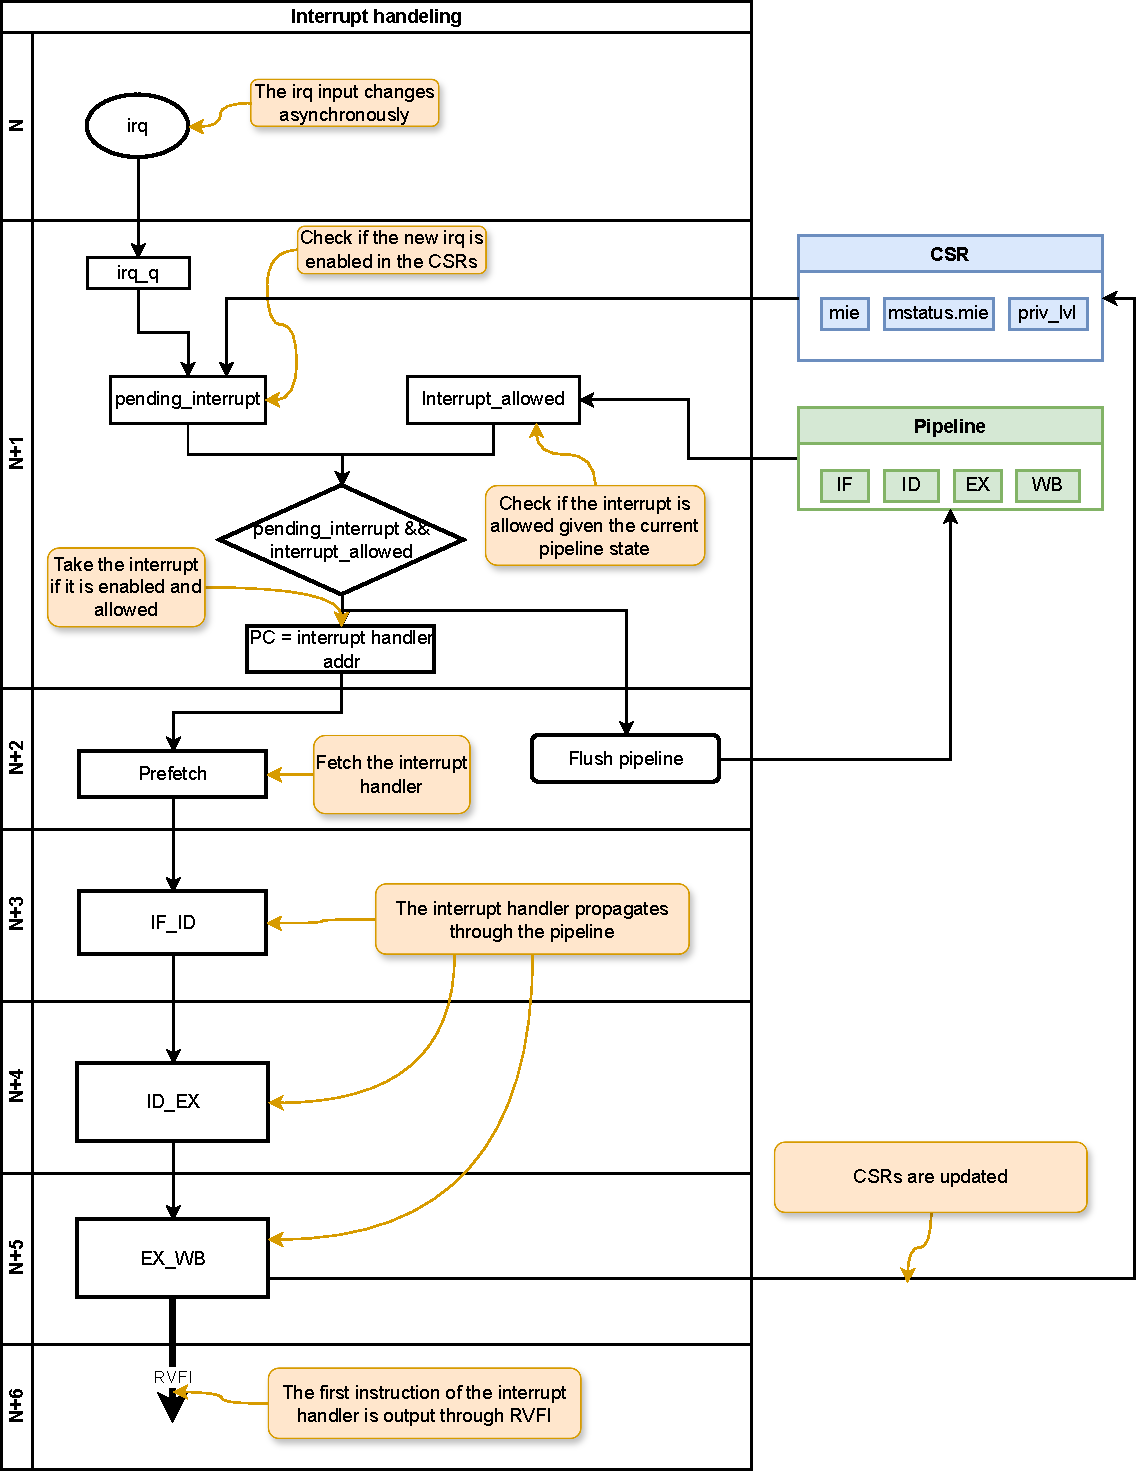
\includegraphics[width=1\linewidth]{figures/interrupt_handeling_timing.pdf}
    \caption{Diagram showing the components that affect the timing of taking an interrupt. The diagram is created by analyzing the RTL code of the CV32E40S~\cite{openhwgroupCv32e40s2024}.}
    \label{fig:interrupt_timing}
\end{figure}






\subsection{Non Maskable Interrupts (NMI)}

\acrfull{nmi} are used only for hardware errors. They can not be disabled and perform a jump to the NMI vector to be handled \cite{watermanRISCVInstructionSet2021}. They update \lstinline{mepc}, \lstinline{mcause}, and \lstinline{mstatus} like normal interrupts, but NMIs are handled in an imprecise manner, allowing the instruction causing the NMI to retire before taking the NMI. At most, two instructions will retire before NMI is taken. 
Also, NMIs are prioritized over other interrupts and will be taken before other pending interrupts \cite{openhwgroupExceptionsInterruptsCOREV2023}.

\subsection{CLIC}

The \textit{Core Local Interrupt Controller (CLIC)} is a more advanced interrupt controller, supporting priority levels of interrupt, nestable interrupts, and up to 4096 interrupts (1024 in CV32E40S) \cite{openhwgroupExceptionsInterruptsCOREV2023}. CLIC's functionality is somewhat different from CLINT's explained above, but the differences are not essential to understanding the complexity of verifying interrupts and will not be discussed further. 



\section{Debug Requests}
\label{sec:bg_debug}

Debug support is an essential part of a processor to allow developers to gain visibility and control of the processor, especially when implemented physically in hardware. CV32E40S supports the RISC-V Debug Specification \cite{pauldonahueRISCVDebugSupport2023} to support low-level debugging access to the processor. The specification defines a standard interface used by a \acrfull{dm} on the RISC-V platform but external to the core. This \acrshort{dm} is further controlled by a Debugger on a Debug Host (e.g. gdb on a laptop), through Debug Transport Hardware (e.g. JTAG), and different transport modules and interfaces. 

The Debug Mode of the core can be entered synchronously through \rv{ebreak} instructions or asynchronously through the \rv{debug_req_i} input signal to the core~\cite{openhwgroupDebugTriggerCOREV2023}.

When the core enters the debug mode, the current PC is saved to the \rv{dpc} CSR, the cause of the debug is saved in the \rv{dcsr} CSR, and the privilege is set in \rv{prv}. The PC is then redirected to a location given in the \rv{dm_haltaddr_i} port, where the processor starts executing the debug control code from ~\cite{openhwgroupDebugTriggerCOREV2023}.

To exit from debug mode, the \rv{dret} instruction is executed, which restores the PC from \rv{dpc} and resumes normal execution at the privilege level set in \rv{prv} and \rv{v}~\cite{pauldonahueRISCVDebugSupport2023}.

\section{Processor Verification Techniques}
\label{sec:bg_verificationTech}

%\textbf{TODO: Compliance vs DV}

A common approach to processor verification is the \textit{step-and-compare} methodology \cite{taylorAdvancedRISCVVerification2023}. Here, the \acrshort{rtl} code of the \acrshort{dut} core runs parallel to a \textit{reference model} in the testbench, like in \Cref{fig:testbench_block_diagram}. They run in \textit{lock-step}, executing the same instructions from a random instruction stream generator or a custom-written directed test. The state of the DUT core and reference model is compared after each instruction \textit{retires}. An instruction has retired when the execution of the instruction has been completed, and all the values of the \acrfull{pc}, \acrfull{gpr}, and \acrfull{csr} are updated \cite{taylorAdvancedRISCVVerification2023}. These signals are output at retirement through a tracer like RVFI, as explained in \cref{sec:rvfi}.

%\subsection{step-and-compare}
%\label{sec:step-and-compare}
The step-and-compare methodology is popular since the state is continuously compared between the DUT and the RM, and there are no wasted cycles after a failure. This is an advantage compared to other methodologies such as post-simulation trace log checking and post-simulation signature checking \cite{duncangrahamRISCVVerificationImplications2023}, where the program has to fully complete before comparing the logs and determining if the test has passed or failed.


For the step-and-compare methodology to be optimal, the reference model should ideally be as independent of the core as possible so that bugs from the core are not also implemented in the reference model.

\subsection{RISC-V Formal Interface (RVFI)}
\label{sec:rvfi}

The RVFI specification is an interface of output signals from the core used to compare execution with the reference model. 
When an instruction is retired from the core, it asserts the \rv{rvfi_valid} signal and outputs the details of the retired instruction and updates to GPR, CSR, PC, etc. \cite{symbioticedaRiscvformalDocsRvfi2020}. It uses signals like \rv{rvfi_rd_addr}, \rv{rvfi_rd_wdata}, \rv{rvfi_rs1_addr}, and \rv{rvfi_rs1_rdata} to describe reads and writes to GPRs, \rv{rvfi_pc_rdata} for the PC, \rv{rvfi_mem_addr, rvfi_mem_wdata,..} for memory operations, etc.

RVFI also supports reporting asynchronous events from the core. In RVFI, interrupts are reported as happening between instructions, so the results from the interrupt will be shown in the first instruction of the trap handler by asserting the \lstinline{rvfi_intr} signals to indicate the interrupt type and cause \cite{openhwgroupRISCVFormalInterface2023}.

This allows the interrupt and debug generators to be connected only to the DUT and the reference model to be alerted of interrupts when reported through the DUT.
This ensures the timing of interrupts stays in sync in the DUT and reference model. However, this also results in the reference model being unable to verify if the DUT takes the interrupts correctly, for instance, when multiple interrupts are present simultaneously \cite{taylorAdvancedRISCVVerification2023}.

\subsection{RISC-V Verification Interface (RVVI)}
\label{sec:rvvi}

\acrfull{rvvi} \cite{riscv-verificationRISCVVerificationInterface2023} is an open verification interface that connects the \acrshort{dut} core and reference model during verification. It provides a standardized way to exchange information about the processor state, executed instructions, and other details. It is divided into the RVVI-Trace and the RVVI-API. The RVVI-Trace extends RVFI and contains the core output, while the RVVI-API adds functions to interface with the reference model. RVVI is intended to be used with a \acrshort{vip}, which contains a reference model as well as comparison functionality. Therefore, the RVVI-API can insert the processor state instead of externally comparing the reference model and \acrshort{dut} core.

\subsection{Direct Programming Interface (DPI)}
\label{sec:bg_dpi}

\textit{\acrfull{dpi}} functions in SystemVerilog provide a way to connect SystemVerilog to other languages like C and \cpp \cite{spearSystemVerilogVerificationGuide2012}. They come in two types: \textit{imported functions} where C/\cpp functions are called from  SystemVerilog, and \textit{exported functions} where SystemVerilog functions can be called from C/\cpp. Using DPI, an ISS written in another language can be used with SystemVerilog. 


\section{Instruction Set Simulators (ISS) }
\label{sec:bg_iss}

An \textit{Instruction Set Simulator (ISS)} is a simulator that simulates the processor execution at an instruction level, fully completing one instruction before moving to the next.
It only takes the RISC-V ISA as a basis and ignores implementation-specifics like the pipeline.
There are many available Instruction Set Simulators for RISC-V, some of which are discussed below.

%\subsection{QEMU}
%\label{sec:qemu}
%
%\textit{QEMU} is an open-source full-system emulator that can run various operating systems on multiple hardware platforms. It supports multiple ISAs, one of which is RISC-V \cite{qemu_project_developers_about_2023}. 
%It uses portable dynamic binary translation to translate full code blocks from one another ISA to RISC-V. QEMU is made to be fast, and multiple optimizations and simplifications are made at the expense of accuracy. For instance, interrupts are not checked at every instruction but at every new code block, so interrupts may be mistimed. \cite{bellard_qemu_2005}
%
%\subsection{Rv8}
%\label{sec:rv8}
%
%\textit{Rv8} is another open-source ISS that uses just-in-time dynamic binary translation, similar to QEMU. Like QEMU, it is also focused on speed, does optimizations at the expense of accuracy, and may be hard to use for verification \cite{clark_rv8_2017}.
%
%\subsection{R2VM}
%\label{sec:R2VM}
%
%The \textit{Rust RISC-V Virtual Machine (R2VM)} \cite{guo_accelerate_2020} is an ISS written in Rust. It utilizes \textit{dynamic binary translation (DBT)} to translate code blocks from the RISC-V ISA to the host's native code. 
%
%The simulator also simulates a 5-stage pipeline. This implementation models the pipeline during the DBT code generation and uses different "hooks" that run at the start of a block, before an instruction, after an instruction, and after a taken branch. The hooks generate microarchitectural simulation code and are used to calculate the number of cycles it takes for an instruction to complete. 
%
%Because the simulator uses DBT, interrupts are checked only at the end of basic blocks since it is difficult to interrupt DBT-ed code \cite{guo_accelerate_2020}. This can be accepted in the R2VM simulator as it is intended for simulating timing, but is not optimal for verification.
%
%
%
%\subsection{riscvOVPsim}
%\label{sec:riscvOVPsim}
%
%\textit{riscvOVPsim} is a free ISS from Imperas. Imperas is a leading processor simulation company. It is instruction-accurate with support for most official RISC-V extensions. It allows configuring the model with different configurations and standard extensions, but riscvOVPsim only works with the standard RISC-V extensions and does not allow users to add custom instructions and extensions without acquiring a license from Imperas. \cite{imperas_software_ltd_risc-v_2023}.
%
%\textit{riscvOVPsimPlus} is an expanded version of riscvOVPsim that adds trace output and a GDB debug interface. It allows an execution log to be output and compared after execution. \cite{imperas_software_ltd_risc-v_2023}


\subsection{Spike}
\label{sec:spike}

\textit{Spike} \cite{SpikeRISCVISA2023} is an open-source functional instruction-accurate ISS written for RISC-V. It is written in \cpp and is relatively simple to use and extend. It is widely used in academia for research and teaching, and in industry as a golden functional reference to multiple RISC-V cores. As the official RISC-V ISS, Spike has been developed alongside the RISC-V specification and is well-tested and maintained. It supports a wide range of RISC-V extensions and allows for the inclusion of custom extensions.

Spike loads ELF binary files containing the instructions to be run. It can be executed sequentially from start to finish or, with some modifications, run in a step-by-step mode, one instruction at a time. 


% Spike revolves around a \lstinline{step()} function in the \lstinline{execute.cc} file that fetches, decodes, and executes an instruction. This is divided into one function \lstinline{_mmu->access_icache(pc)} that fetches an already decoded instruction (with \lstinline{decode()}) with the type \lstinline{insn_fetch_t}, and either run \lstinline{execute_insn_fast()} or \lstinline{execute_insn_logged()} to execute the instruction quickly or slowly with logging. In Spike, the execute functions also write the results to the simulated register file \cite{SpikeRISCVISA2023}.


%Pure spike runs from \lstinline{spike.cc} in the main function. The main execution is done by instantiating a \lstinline{sim_t} that gets configured with the processor and memory. The construction in \lstinline{sim_t} instantiates a configurable amount of \lstinline{prcessor_t} processor types. The original implementation from main fully runs Spike until completion using the \lstinline{sim_t::run()} function.

%\lstinline{sim_t} has a method called \lstinline{step()} that steps through a given number of instructions in each of the configured processors. 


\subsection{Sail-riscv}
\label{sec:sail}

\textit{Sail-riscv} \cite{RISCVSailModel2023} is a model of RISC-V written in the Sail language. The Sail language is specifically designed for specifying \acrshort{isa}s for a processor. It is intended to precisely define the ISA to avoid ambiguity of an ISA specification written in text or pseudocode \cite{armstrongSailInstructionsetSemantics2023}. The Sail code can generate latex documentation, type checking, theorem prover definitions, and executable emulators in C.  

Sail-riscv is the sail specification for RISC-V and has been adopted as the golden formal model by the RISC-V Foundation. 
The C-emulator generated from the sail-riscv model makes it possible to use the model as an ISS. The emulator mixes autogenerated code from the sail model with handwritten wrapper code. The generator can be configured to use different extensions, and custom extensions written in Sail can also be included in the simulator. 

%Sail-riscv also revolves around a \lstinline{step()} function. Inside the step function, instructions are fetched with the \lstinline{fetch()} function, decoded with \lstinline{ext_decode()}, and executed with \lstinline{execute()}. Execute also writes the data back to the register file and executes side effects. \cite{RISCVSailModel2023}


%\begin{itemize}
%  \item Emulator generated from the risc-v sail specification.
%  \item the c emulator is an interpreter. Fetches and decodes instructions from emulated ram. \cite{}
%  \item Supports RVFI\_DII (Risc-V Formal Interface - Direct Instruction Injection)
%  \item Supports RV32I, RV64I, M, A, C, F, D, Zicsr and N extensions
%  \item \textbf{Lacking} support for multiple extensions: E, Zmmul, Zicntr, Zihpm, Zifencei... 
%  \item openHW has been considering implementing these in sail \textbf{but unclear what the status is}. 
%  \item base counters and timers
%  \item Machine-level and supervisor-level
%  \item supports CLINT
%\end{itemize}


%\section{Micro-Architectural simulators}
%
%Micro-architectural simulators simulate computer systems by modeling the different underlying hardware components, achieving cycle-accurate simulation \cite{akram_survey_2019}. Some micro-architectural simulators will be introduced below.
%
%
%\subsection{Gem5}
%\label{sec:gem5}
%
%\textit{Gem5} is an open-source architecture simulator. It decouples the ISA semantics from the CPU model, allowing the simulation of multiple ISAs and CPU models. It has support for atomic, in-order, and out-of-order CPU models, and recently received support for RISC-V \cite{roelke_risc5_2017} \cite{hin_supporting_2021} \cite{lowe-power_gem5_2020}. 
%
%Gem5 is popular for architectural exploration but lacks some features that might be necessary for verification. For example, it lacks support for running in lock-step execution, lacks a trace output for each cycle, and is non-trivial to add custom instructions and extensions.
%
%While Gem5 is cycle-accurate, significant modifications to the included prebuilt CPU models are necessary to represent the DUT core accurately. 
%
%Gem5 is actively developed and maintained and is likely to continue getting support. \cite{noauthor_gem5_2023}
%
%%\begin{itemize}
%%    \item Open source architecture simulator
%%    \item Hardware is black boxes with tunable latencies and attributes
%%    \item Multiple CPU models; atomic, in-order, out-of-order
%%    \item Decouples ISA semantics from the CPU models
%%    \item Might be slow compared to other ISS alternatives
%%    \item Syscall Emulation (SE) mode simulation or Full System (FS) mode simulation
%%\end{itemize}
%%
%%Gem5 is intended for performance evaluation, so to use it for validation, some work has to be done.
%%We need to support:
%%
%%\begin{itemize}
%%    \item Lock-step execution
%%    \item trace output for each cycle
%%    \item Ability to supoprt custom extensions and instructions
%%    \item Modify the cpu model to resemble the core to be simulated.
%%    \item Modularity in choosing RISC-V extensions
%%\end{itemize}
%
%%Gem5 is more complex than Spike and Sail, but might be harder to modify without altering side effects
%%
%%Gem5 might lead to more work to modify and/or might be more messy.
%%
%%Could become too similar to the RTL, and possibly have the same bugs.
%
%
%%\subsection{TinyEMU}
%%
%%\begin{itemize}
%%    \item System emulator
%%    \item Small and simple
%%\end{itemize}
%
%\subsection{MARSS-RISCV}
%\label{sec:marss}
%
%\textit{MARSS-RISCV} is an open-source cycle-level micro-architectural simulator for RISC-V, built on top of the TinyEMU emulator. It has cycle-level models for both in-order and out-of-order pipelines, configurable with 5-stage- and 6-stage pipelines \cite{kothari_marss-riscv_2019}. It is also intended for full system simulation, performance evaluation, or architectural exploration, not verification.
%
%It currently only supports the RV32GC and RV64GC ISA extensions. The last commit to the project was 3 years ago (Dec 9, 2020), and it has multiple reported unfixed bugs that are several years old.
%
%To simulate the pipeline, the simulated core has a \lstinline{CPUStage} object for each pipeline stage, with info about the stage. Among other things, it holds an \lstinline{InstructinoLatch} object that serves as a placeholder for a single instruction, containing the decoded instruction and other information about the instruction that is updated as it moves through the pipeline \cite{gaurav_kothari_marss-riscv_2020}.
%Each pipeline stage also has a function responsible for running the stage and moving the instruction placeholder to the next stage if allowed. To ensure stalls are considered, the functions are run in reverse order, from WB to IF.
%
%
%%\begin{itemize}
%%  \item cycle-level
%%  \item Multi core
%%  \item Written in rust
%%  \item 5 stage in-order pipeline
%%  \item Mostly focused on performance and simulating timing of pipeline.
%%  \item Interrupts only handled at the end of code blocks.
%%\end{itemize}

\section{Existing RISC-V Reference Model Solutions}
\label{sec:bg_existingReference}

Reference models can have varying complexity, from simple  \acrshort{iss}s to more advanced cycle-accurate models. This section will cover a few existing RISC-V reference model solutions.

\subsection{ISS as a Reference Model}
\label{sec:bg_iss_refmod}

An ISS is often used directly as a reference model. This requires modifications to how asynchronous events are handled in the testbench, as shown in \Cref{fig:iss_testbench}. To avoid the timing problems of asynchronous events shown in \Cref{fig:lw_example}, interrupts and debug requests are only passed into the DUT core, not the ISS. The ISS is instead informed of asynchronous events through the RVFI output of the core and takes the same asynchronous events that the core reports. Since the interrupts follow the core, this leaves a large "verification hole" where we can not verify if the correct asynchronous event was taken or if it was taken at the correct time \cite{taylorAdvancedRISCVVerification2023}. 

\begin{figure}
    \centering
    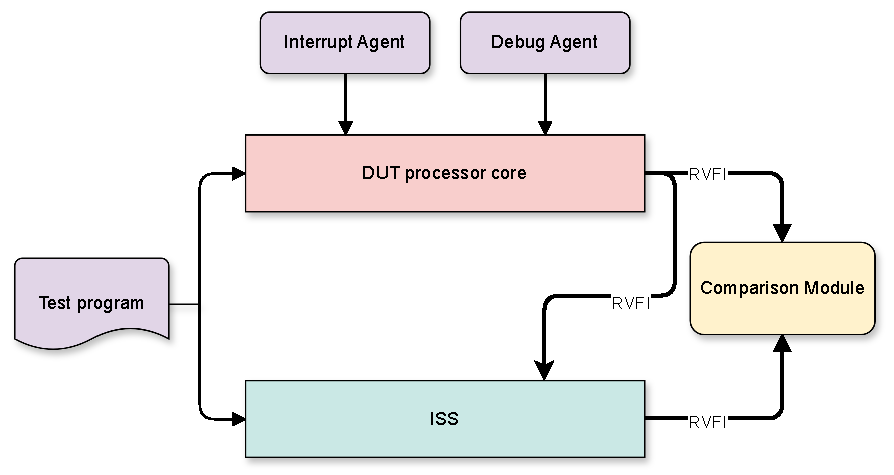
\includegraphics[width=0.75\linewidth]{figures/ISS_architecture.pdf}
    \caption{Testbench architecture when using an ISS as the reference model.}
    \label{fig:iss_testbench}
\end{figure}
%\subsection{riscvOVPsim}
%
%OVPsim was used in the core-v-verif verification environment before switching to ImperasDV using the step-and-compare methodology. The RVFI output from the core was monitored by an RVFI monitor, which determined the instruction type. An RVVI driver was responsible for driving the reference model using the different RVVI-API functions. The \lstinline{stepi(REQ req)} function was used to step the reference model in normal execution. When an interrupt occurred in the DUT, \lstinline{stepi_ext_intr(rvvi_ovpsim_seq_item.intr_id)} or \lstinline{stepi_nmi_load_fault()} was used to notify the riscvOVPsim of the interrupt \cite{openhwgroupOpenhwgroupCorevverif2023}.

The Spike ISS has been used as a reference model in multiple RISC-V cores, and some of the implementations are described below.

\subsubsection{CVA6 Spike Tandem Reference Model}
\label{back:cva6}

CVA6 is another core from the OpenHW Group and uses the same \textit{core-v-verif} verification environment as the CV32E40S core, with some modifications. A tandem verification approach with Spike is currently being developed to verify the CVA6 core, using Spike with some modifications as a reference model.

The implementation revolves around the \lstinline{step()} function in Spike, which is expanded to output an RVFI item after running a step. This is passed to the scoreboard in the verification environment, where it is compared to the DUT. The \lstinline{spike_step()} function is called from the verification environment as a SystemVerilog DPI function and executes the \lstinline{step())} function in Spike \cite{openhwgroupOpenhwgroupCorevverif2023}.

Interrupts are reported from the DUT through the RVFI interface as described in \cref{sec:rvfi}. This way, the interrupts are taken at the same instruction in the DUT and Reference Model, but it can not verify if this is the correct time to do so.

Certain sections in the RISC-V ISA specification use terms like "may" or "can". This ambiguity has led to discrepancies between the Spike Reference Model and the CVA6 core due to differences in the interpretation of the specification. There is ongoing work to find these discrepancies \cite{CVA6CSRSpike} and patch Spike to operate the same way as the CVA6 core. 


\subsubsection{Spike Co-simulation in the Ibex RISC-V Core}
\label{back:Ibex}

Ibex is another open-source RISC-V core from lowRISC. It currently uses Spike for co-simulation and verification. It uses a step-and-compare-based approach, but instead of outputting the changed processor state through RVFI to a separate compare module, Spike is extended to compare Spike against the DUT changes internally. Spike has also been expanded to take the RVFI item from the DUT as input and use this for comparison. To inject interrupts into Spike, the added functions \lstinline{set_nmi()}, \lstinline{set_mip}, \lstinline{set_debug_req} are called from over DPI from \lstinline{ibex_cosim_scoreboard.sv}.
Ibex also extends RVFI with the \lstinline{rvfi_ext_irq_valid} signal to report an interrupt not associated with an instruction, not setting \lstinline{rvfi_valid}. This keeps the order of the interrupts correct in comparison to the retired instructions instead of passing interrupts independent of RVFI. This also allows multiple interrupts to happen between two instruction retirements \cite{ethzurichanduniversityofbolognaCosimulationSystem2023}. 

%\begin{itemize}
%    \item Uses Spike as an ISS for cosimulation
%    \item Does not extend to 
%    \item When the DUT receives an interrupts and sends this in the rvfi item, this is sent to Spike using \lstinline{set_nmi()}, \lstinline{set_mip}, \lstinline{set_debug_req} etc. in \lstinline{ibex_cosim_scoreboard.sv}
%    \item Extends rvfi with \lstinline{rvfi_ext_irq_valid} to signal an interrupt not associated with an instruction, not setting \lstinline{rvfi_valid}. This keeps the order of the interrupts correct in comparison to the retired instructions, instead of passing interrupts independent of RVFI. This also allows multiple interrupts to happen between two instruction retirements.
%    \item Interrupts follows the DUT, leaving a verification hole
%    
%\end{itemize}


\subsection{ImperasDV}
\label{sec:imperasdv}

ImperasDV is a more advanced \acrfull{vip}, compared to the simpler ISS implementations above. This implements the RVVI-API and contains a reference model, comparison tools, a scoreboard, and other verification components. By integrating the comparison process into the VIP, ImperasDV gains better control when verifying asynchronous events compared to a simpler ISS implementation~\cite{taylorAdvancedRISCVVerification2023}. 

While the internal workings of ImperasDV are proprietary, we can use the surrounding implementation and output logs \cite{ISSMismatchPending2023} to make assumptions about how it might work to compare it to the solution explored in this thesis.

ImperasDV uses the RVVI-API to pass retired instructions from the DUT to the VIP. When an interrupt or other asynchronous event is applied to the DUT, the \textit{net changes} (signals that have changed) are pushed to ImperasDV with the \lstinline{rvvi.net_push()} function. ImperasDV then analyzes all the legal sets of actions to determine if any of them converge to the provided DUT state. 
It explores different orderings of applying legal net changes and executes until an instruction retires. It then compares the state changes of ImperasDV with the state changes of the DUT. If no state changes match the DUT, an error is thrown, indicating that the DUT made an illegal state change.

\Cref{fig:imperasFork} shows an example of how we imagine different states are explored and is generated by analyzing an output error log from ImperasDV \cite{ISSMismatchPending2023}. The figure shows how ImperasDV applies net changes in various combinations of orders and runs until retirement. The example shows the two net changes, setting \rv{haltreq => 0} and \rv{nmi_cause => 0x401}, as well as an exception. 

This is an improvement from the ISS method described in \Cref{sec:bg_iss_refmod}, as interrupts no longer follow the DUT, taking the same interrupts that the DUT reports it has taken. Instead, ImperasDV verifies that the state transition of the DUT is legal. Although this is an improvement, it still leaves some holes in the verification coverage.
ImperasDV still has no pipeline awareness and can only verify that the DUTs state transition is legal, but not whether it was the correct legal state change considering the pipeline content \cite{taylorAdvancedRISCVVerification2023}.

\begin{figure}
    \centering
    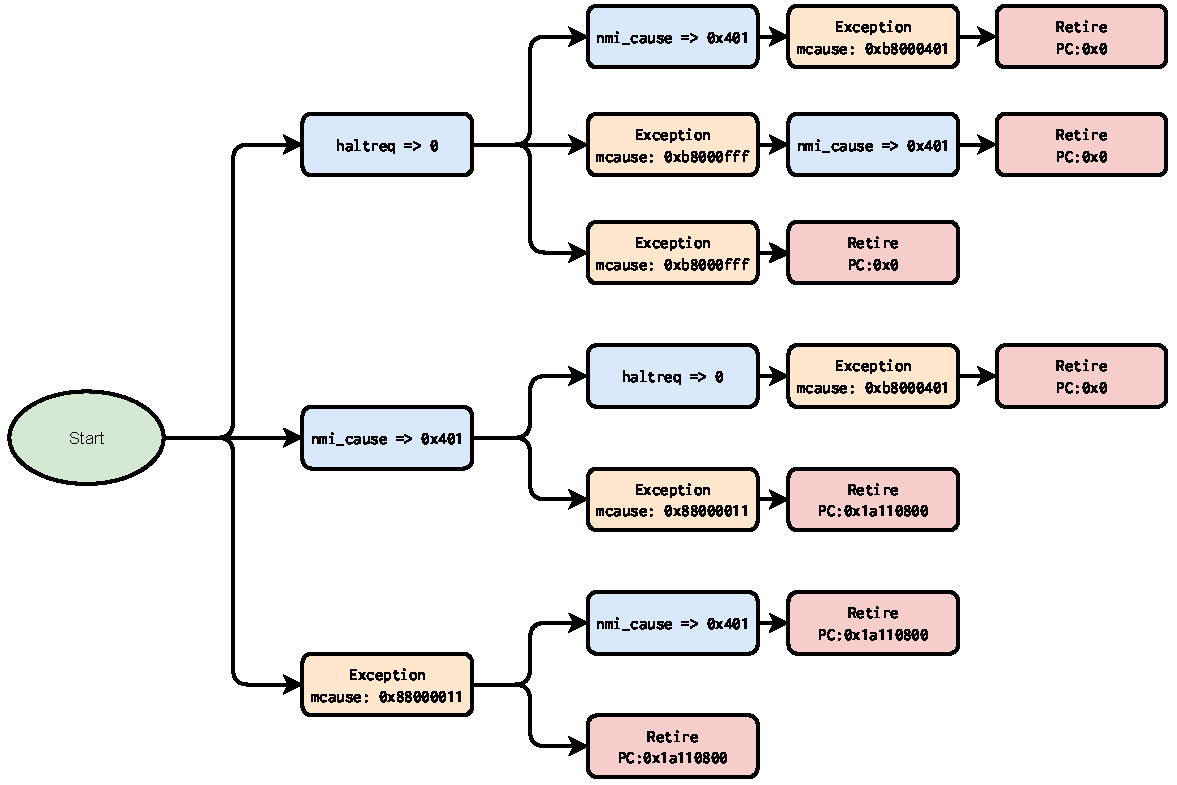
\includegraphics[width=1.0\linewidth]{figures/ImperasExecution.pdf}
    \caption{Diagram showing how ImperasDV explores different variations of net changes in "fork" design. Figure based on error log from \cite{ISSMismatchPending2023}. }
    \label{fig:imperasFork}
\end{figure}

%\subsection{Onespin RISC-V}
%
%Onespin has a RISC-V verification solution OneSpin RISC-V Integrity Verification Solution. \cite{onespinsolutionsAssuringIntegrityRISCV2019} 
%This works by formalizing the ISA into a set of SystemVerilog Assertions.
%
%formal and simulation friendly
%
%Each instruction is translated to a single operational assertion that can map to sequential or pipelined implementation \cite{onespinsolutionsAssuringIntegrityRISCV2019}.
%
%Used to verify the Rocket Core with all instructions, privilege levels, interrupts and exceptions mapped into assertions \cite{onespinsolutionsAssuringIntegrityRISCV2019}.
%
%To implement this approach, it would require the model to be fully described using assertions.




\section{Core-v-verif, the CV32E40S Verification Environment}
\label{sec:bg_core-v-verif}

\textit{core-v-verif} \cite{openhwgroupOpenhwgroupCorevverif2023} is the verification environment used by the CV32E40S core, as well as other OpenHW cores. This allows many similar verification components to be reused by different cores, which avoids all core developers having to do overlapping work.

Currently, core-v-verif uses ImperasDV as its primary reference model, implementing the Continuous Compare Lock-Step Co-Simulation approach \cite{duncangrahamRISCVVerificationImplications2023}, and is shown in \cref{fig:cv32e40s-overview}. In this approach, the interrupt and debug generators are only connected to the DUT, and the reference model is informed of interrupts through the RVFI and RVVI interface. 
The testbench either runs custom-written directed tests or uses randomly generated test programs using the \textit{corev-dv} Random Instruction Generator
\cite{openhwgroupOpenhwgroupCorevverif2023}.

The DUT uses an \textit{RVFI (Risc-V Formal Interface)} tracer interface to report the internal status of the core \cite{symbioticedaRiscvformalDocsRvfi2020}. This is fed to the RVVI Driver on every instruction retirement or interrupt/trap. Additionally, asynchronous net changes are also reported to ImperasDV using the RVVI-API. This is used in ImperasDV to compare the result from the DUT to the result from the Reference Model. 


\begin{figure}
    \centering
    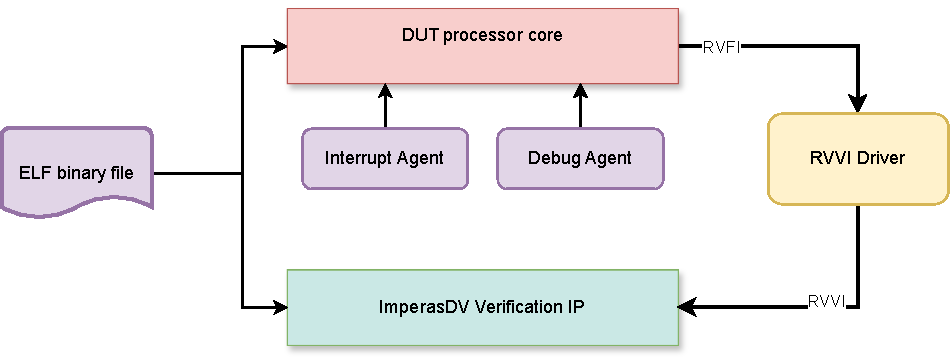
\includegraphics[width=0.75\linewidth]{figures/core-v-verif.pdf}
    \caption{Overview of the verification environment for the CV32E40S core based on figure from \cite{openhwgroupOpenhwgroupCorevverif2023}.}
    \label{fig:cv32e40s-overview}
\end{figure}



%The full list of RVFI signals for the CV32E40S core can be found in \cite{openhw_group_risc-v_2023}, but some useful signals are listed below.
%
%\begin{itemize}
%    \item \lstinline{rvfi_insn} - The retired instruction word
%    \item \lstinline{rvfi_trap} - Signals that a synchronous trap has occurred, like a trap, exception, debug, etc.
%    \item \lstinline{rvfi_intr} - Signals that an interrupt has occurred, with the cause.
%    \item \lstinline{rvfi_pc_rdata} - PC of the retired instruction
%    \item \lstinline{rvfi_pc_wdata} - Next predicted PC. Ignores asynchronous traps
%    \item \lstinline{rvfi_csr_...} - Control and status register
%    \item \lstinline{rvfi_gpr_...} - The general purpose registers (x0-x31)
%    
%\end{itemize}



\section{The Problems with Using an ISS as a Reference Model}
\label{sec:back_issProblem}

%All the implementations from \cref{sec:bg_existingReference} except ImperasDV use an ISS as a reference model.
\textcite{taylorAdvancedRISCVVerification2023}  discuss multiple problems when using an ISS as a reference model. The first problem is the difference in abstraction level between the DUT and the ISS. On one hand, the DUT is typically simulated at a clock-cycle accurate Register Transfer Level. On the other hand, ISSs are simulated with time modeled at the instruction level, with the cycle timing of memory interfaces and pipeline operation abstracted away. This leads to an inconsistency between the two. For instance, the RTL model might take multiple clock cycles to complete an instruction while the ISS executes it in one cycle.

When there are no asynchronous events, the ISS can accurately predict the execution of instructions. The problem arises with asynchronous events. In an instruction-accurate simulator, interrupts and debug requests are seen as happening at the beginning of a new instruction. In contrast, they could occur in the middle of a multi-cycle instruction. In addition, the ISS does not know the state of the pipeline. In some cases, as explained in \cref{sec:bg_pipeline}, the pipeline has states where interrupts can not immediately be taken, causing a mismatch where the ISS takes the interrupt before the DUT.

We highlight this problem in \Cref{fig:lw_sw_pipeline}, which shows the same example as \Cref{fig:lw_example} but shows the pipeline content of the CV32E40S core while executing the instructions. It shows the PC and instructions for the IF, ID, EX, and WB stages and blank spaces where the instructions are invalid. The IA (Interrupt Allowed) column also shows whether an interrupt can be taken, given the current pipeline state. In CV32E40S, an interrupt can not be taken if there is an outgoing memory request to the \acrshort{lsu}~\cite{openhwgroupExceptionsInterruptsCOREV2023}. In this example, this is the case when a load or store instruction is in the EX or WB stages. These cases are highlighted in red, showing that the interrupt can not be taken. An external interrupt is applied when interrupts are not allowed, and we see that the interrupt is only taken after the \sv{interrupt_allowed} signal goes high. Since the ISS in \Cref{fig:lw_example} does not know the content of the pipeline, it takes the interrupt immediately after the interrupt is applied.

\begin{figure}
    \centering
    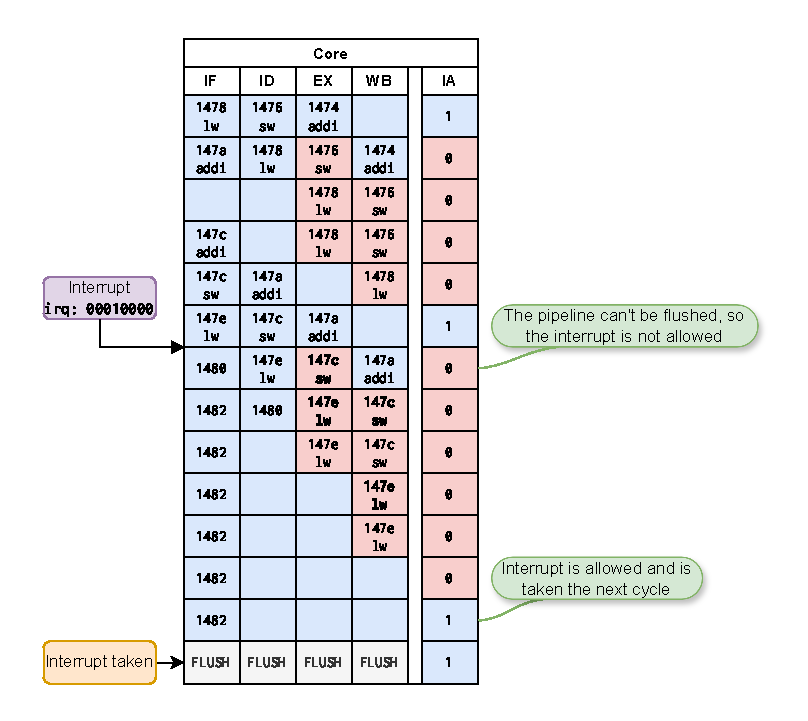
\includegraphics[width=1.00\linewidth]{figures/lw_sw_pipeline_example.pdf}
    \caption{Example showing how load and store instructions in the pipeline prohibit an interrupt from being taken.}
    \label{fig:lw_sw_pipeline}
\end{figure}


Another problem discussed is the timing of \textit{side effects}, which are state changes not explicitly part of the instruction \cite{taylorAdvancedRISCVVerification2023}. Typically, this can be predicted with an ISS in normal execution, but they can be inaccurate when asynchronous interrupts are introduced, where the pipeline execution can alter the timing of the side effects.









%This has typically been done with the "step-and-compare" methodology, where the DUT runs until an instruction retires, then the RTL clock is stopped and the reference model is run until it also retires an instruction. At this point, the testbench compares the states in the DUT and RM before starting the RTL clock again.

\section{Cycle-accurate Modeling Techniques}
\label{sec:bg_cycle-accurate}

Multiple approaches for cycle-accurate modeling have previously been attempted for different processors and instruction set architectures.

\textcite{chiangEfficientTwolayeredCycleaccurate2009} proposed a two-layered cycle-accurate modeling technique that partitions the simulator into an untimed functional kernel and an outer timing shell. The inner functional kernel is essentially an untimed ISS responsible for executing the instruction and calculating the correct register values, outputs, and memory data.

The timing shell is shown in \cref{fig:timeshell}, sits on top of the functional kernel, interacts with the rest of the system, and updates the changes calculated in the functional kernel at the correct time. The timing shell consists of a commander that takes in external inputs, checks the internal processor state, and determines whether there should be a stall. If the processor should not stall, the commander either sends a \textit{step} or \textit{interrupt} command to the functional unit according to the inputs and receives a result packet when the functional unit has completed. The result goes into the scheduler, which correctly times the updates from the result packet to the correct clock cycle in the time wheel described below. To place updates correctly into the time wheel, the scheduler needs to know all the implementation details of the processor. This includes what happens in each pipeline stage, dependencies between instructions, instruction cycle timing, hazard detection, and stall/forwarding functionality. 

The time wheel consists of multiple time slots corresponding to specific clock cycles and holds all the data to update the outputs and registers at the correct clock cycle. Because of the processor pipeline, one instruction might need to update multiple time slots if the instruction has side effects in different stages. It also has a field indicating if the cycle should stall or not, in which case no command packet is sent to the functional kernel. The time wheel advances each clock cycle, and the most recent time slot is executed.

Another cycle-accurate model is the FaCSim, a fast and cycle-accurate architecture simulator by \textcite{leeFaCSimFastCycleAccurate2008} that follows a strategy similar to Chiang and Huang's. FaCSim also consists of a functional simulator and a Cycle-Accurate Trace simulator with a slightly different approach. The functional simulator is responsible for fetching, decoding, and executing instructions. It generates an execution trace stored in a circular queue connecting the functional and cycle-accurate simulators. 

The execution trace consists of the fetched instruction, the EX stage execution latency, memory traces, etc. The functional simulator also keeps track of pipeline interlocks and simulates stalls by inserting empty bubble instruction trances to simulate stalls from hazards and branches.

Instead of performing cycle-by-cycle instructions simulation, the simulator computes the elapsed cycles in each pipeline stage and adds them up to advance the clock. 

The cycle-accurate simulator loads instruction traces from the circular queue and passes them through the pipeline. Each pipeline stage has a corresponding function that calculates the delay for each stage. After calculating the delay for all stages, the core clock is updated after the writeback stage. 

\begin{figure}[htb]
    \centering
    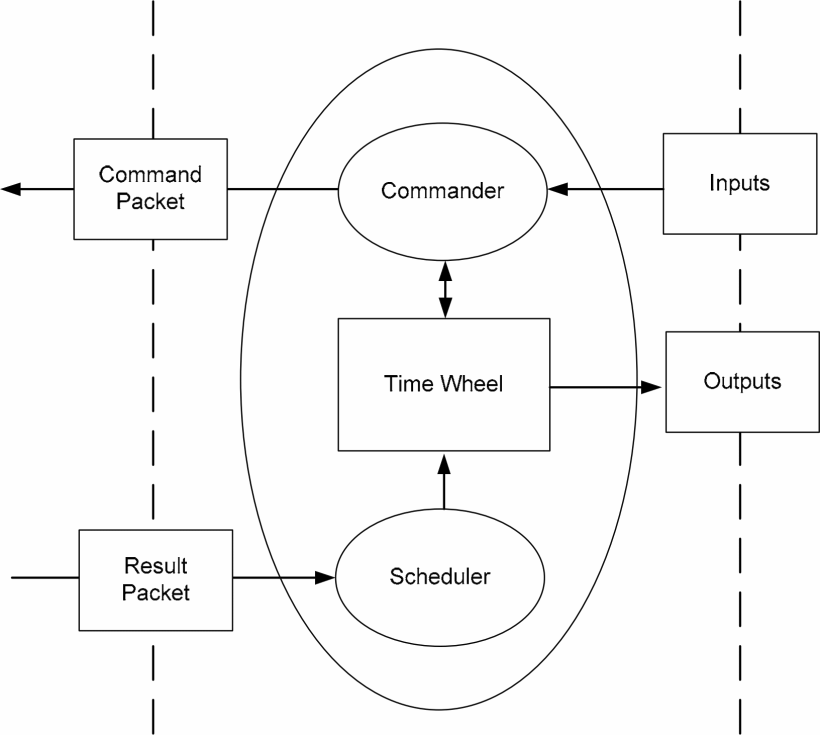
\includegraphics[width=0.5\linewidth]{figures/timeShell.png}
    \caption{Architecture of the timing shell from \cite{chiangEfficientTwolayeredCycleaccurate2009}.}
    \label{fig:timeshell}
\end{figure}

\section{Formal Verification}
\label{sec:bg_formal}

\acrfull{fv} is a powerful technique in verification that uses mathematical tools to analyze the entire space of possible behaviors of a design instead of simulating particular values \cite{seligmanFormalVerificationEssential2015}. Instead of running many simulations to cover all corner cases, formal verification can mathematically prove whether the properties of a design hold for all possible states.

FV has many advantages over simulation-based verification. Since it can mathematically prove whether a property holds or not, we can know for a fact that the property will always hold. In simulation-based verification, we can only know that the property holds for the specific conditions tested throughout many tests, but we can not be sure that every condition is tested. FV can also find corner cases the designer never considered and evaluate infinite behavior to guarantee whether a state is ever reachable.
Additionally, FV can generate minimal examples highlighting where a property fails, simplifying debugging compared to simulation-based verification, where the cause of a failure may have to be identified within a simulation of thousands of random instructions \cite{seligmanFormalVerificationEssential2015}.

Validating a design with \acrshort{fv} requires a \textit{specification} and an \textit{implementation}. The specification is often a more abstract description of the design requirements in the form of properties like \acrfull{sva}, an \acrshort{rtl} model, or a high-level model, while the implementation is usually \acrshort{rtl} code \cite{seligmanFormalVerificationEssential2015}. 


\subsection{Assertion-Based Verification (ABV)}

\acrfull{abv} is a technique where assertions \acrfull{sva} are used to describe properties of the \acrshort{rtl} code \cite{seligmanFormalVerificationEssential2015}. In \acrshort{abv}, properties expressed with \acrshort{sva} can sometimes fully describe the specification of a design. \acrshort{abv} can be implemented in formal verification and simulation.

\subsection{SystemVerilog Assertions (SVA)}

An assertion is an expression or property expected to be always true in a design \cite{mehtaSystemVerilogAssertions2020}. If it is false, we expect to see an error. 
\acrfull{sva} is a \textit{Formal Specification Language} part of the SystemVerilog language used to define design properties precisely. It can be used both in formal verification with \acrfull{abv} and with simulation-based verification \cite{cernySVAPowerAssertions2015}.

\subsection{Formal Equivalence Verification}

\acrfull{fev} is a formal verification tool that compares the RTL code to a reference model \cite{seligmanFormalVerificationEssential2015}. \acrshort{fev} is often used to compare two \acrshort{rtl} models to ensure they are equivalent. To use \acrshort{fev}, both RTL models must be behaviorally equivalent at every cycle.

\textit{Sequential equivalence verification} verifies if two models will generate the same result after the same time with equal inputs. The internal state elements do not have to be identical, only the outputs \cite{seligmanFormalVerificationEssential2015}.

%If sequential \acrshort{fev} tools are available, \textcite{seligmanFormalVerificationEssential2015} recommends using these tools instead of writing properties if the reference model is complete enough. However, tools for sequential \acrshort{fev} are still limited, especially for comparison with higher-level models.

\subsection{Equivalence Checking using Assertion-Based Verification}
\label{sec:bg_eq_abv}

Although \acrshort{abv} is most commonly used where the properties expressed with assertions serve as the reference itself \cite{seligmanFormalVerificationEssential2015}, assertions can also be used for equivalence checking between two models \cite{kumarEquivalenceCheckingUsing2015}. By using \acrshort{sva} to compare the outputs of two models, we get more control over which signals to compare and when to compare them. This is useful if we build a reference model with a higher abstraction level that is not fully behaviorally equivalent at every cycle, which is required for \acrshort{fev}.


\subsection{Onespin 360}

Onespin 360 \cite{onespinsolutionsgmbhUserManualOneSpin} is one of the available proprietary formal verification tools and will be used for the formal verification part of this thesis. Among other things, Onespin has a \textit{Module verification} mode, which uses \acrshort{abv} to do property checking on the design, using \acrfull{sva}.

